
%----------------------------------------------------------------------------------------
%	THE METHODS
%----------------------------------------------------------------------------------------

\headerbox{Experiment}{name=experiment,column=0, below=assumptions
%,row=0, bottomaligned=assumptions
}{
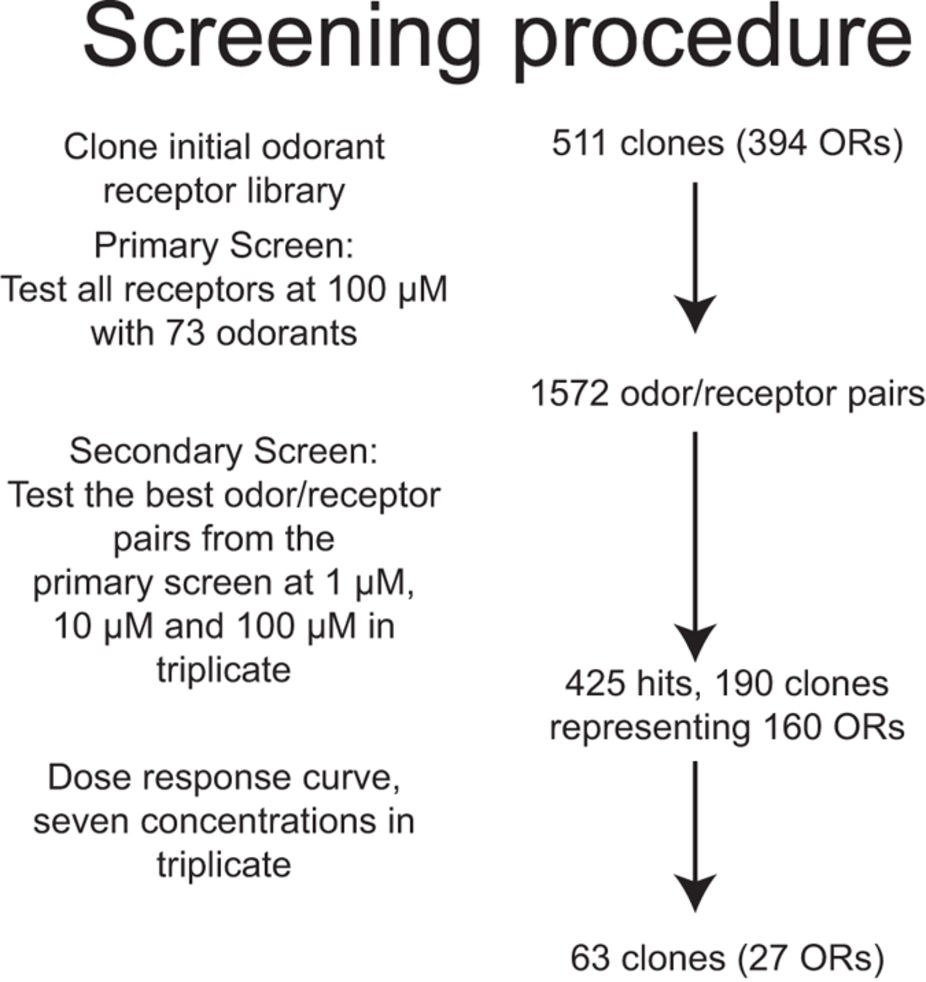
\includegraphics[width= 0.49 \textwidth]{fig/mainland_flow.jpg}
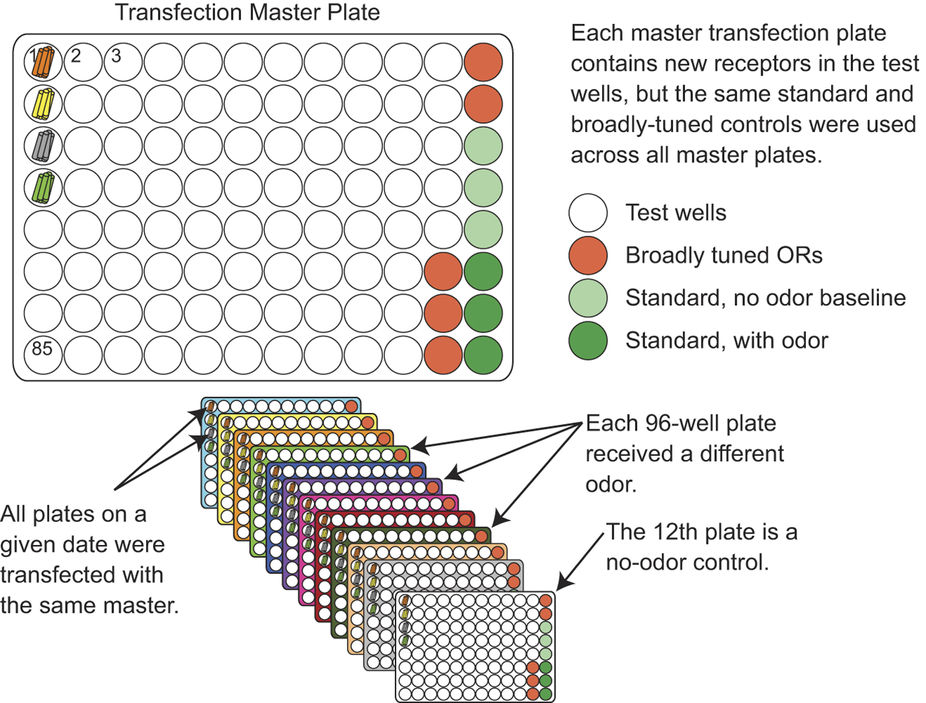
\includegraphics[width = 0.49 \textwidth]{fig/mainland_primary.jpg}

Figure and data from Mainland et al \cite{mainland}
%Now we know the preferred volume $v_n$ of each receptor and also its flexibility $\sigma_n$.
}

\headerbox{To Normalize or Not to Normalize}{name=normalize,column=0, below=experiment, above=bottom
%,row=0, bottomaligned=assumptions
}{
The experiment gives two numbers per well, 
one measures the cell response to odorant ($Luc$) 
and the other one reports the transfection efficiency, cell death and etc ($RL$).
It is assumed that $Luc \propto RL$ for a given condition (eg, the same concentration of odorant),
so the readings are normalized in the following way:
\[r = \frac{Luc}{RL}\]

But in practice, it does not work ..., 
We think that this is a better choice:
\[r = \frac{Luc}{<Luc_{test, c=0}>}\]
This assumes that cells are uniformly distributed among wells. 
%Now we know the preferred volume $v_n$ of each receptor and also its flexibility $\sigma_n$.
}
